%!TEX root = ../doc.tex
\chapter{Implementation}
\label{sec:Implementation}
This Chapter describes the implementation and the connections of the individual components of the augmented reality system. 
\section{Hardware}
\label{sec:Hardware}
The following section describes the evaluation and setup of the hardware used for the camera head and the processing system.
\begin{figure}[H]
    \centering
    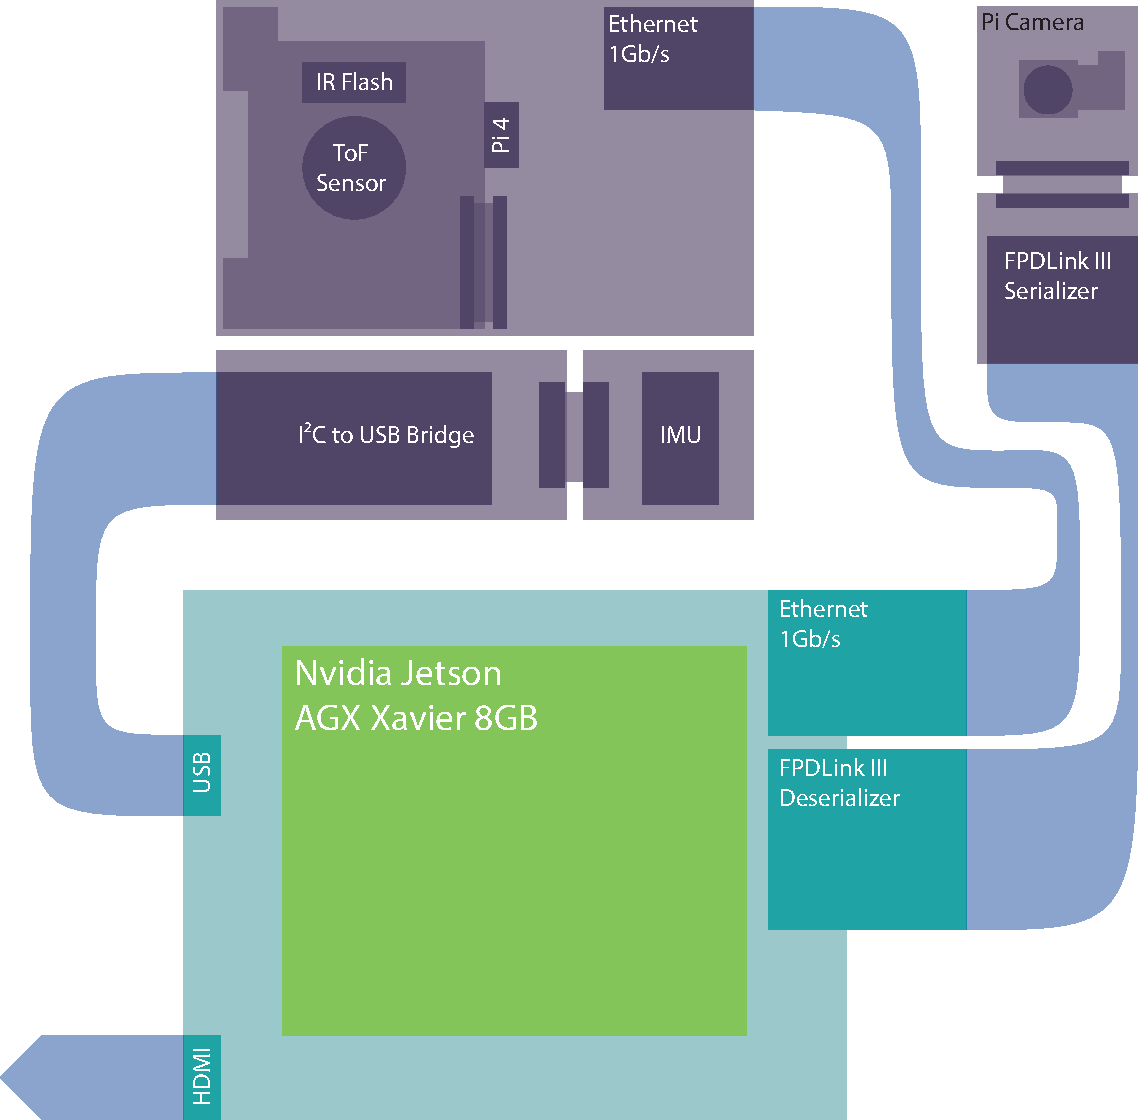
\includegraphics[width=1.0\textwidth]{images/hardware.pdf}
    \caption{Hardware overview. The purple objects belong to the camera head, which is connected to the processing system in cyan.}
    \label{fig:HW_diagram}
\end{figure}
\subsection{Evaluation of ToF Camera}
\label{sec:CamEvaluation}
For the evaluation of the ToF camera, cost and availability have been the main factors in the evaluation, with it being directly CSI-2 connected being an important feature.\\
Internet research has shown a handful of different sensors powering multiple products of diverse manufacturers in varying price ranges. \\
\\
\textbf{Infineon REAL3 IRS1125 (Chosen)}\\
The Infineon IRS1125 ToF Sensor is available in a USB-based development kit by pmdtec – an integrator for ToF technology into smartphones – and on the affordable PiEye Nimbus 3D camera, which is sold as a Raspberry Pi accessory and used in this thesis.\\
The sensor features a resolution of 352x288 pixels at 30 frames per second in the variant IRS1125A. The variant IRS1125C – used by pmdtec – allows 60 frames per second. The pmdtec development kit is tuned for measuring up to 6 meters, while the PiEye camera is limited to 5 meters.\\
While both camera systems are available to be shipped, the pmdtec pico monstar costs about 1500 US Dollars; in contrast, the PiEye Nimbus costs only 230 Euros. The PiEye company advertises its camera with open source software to embed it into the Raspberry Pi ecosystem. However, further investigation has shown that the middleware – the library managing the camera’s settings and connecting to the video4linux2 framework – is still under NDA with Infineon. \\
With a lightweight TCP/IP protocol, the PiEye module is suitable with a Raspberry Pi, acting as a Gigabit Ethernet camera. The PiEye Nimbus is the module of choice for this thesis – the availability, the price, and the specifications are all reasonable. The options to reverse engineer the middleware or sign an individual NDA with Infineon have been kept open initially but were not necessary as the Gigabit Ethernet implementation worked well enough.\\
\\
\textbf{Sony DepthSense IMX556PLR}\\
The Sony IMX556PLR ToF Sensor offers a resolution of 640 x 480 pixels at 30 frames per second and is used by Basler, Lucid Vision Labs, and DephtEye, primarily for Gigabit Ethernet cameras. The IMX556PLR seems to be the most capable ToF sensor freely available in off-the-shelf products at the time.  \\
The technically most compelling product for this thesis would have been the Helios Flex by Lucid Vision Labs, which directly connects via CSI-2 and is sold specifically for use on an Nvidia Jetson TX2 Developer Kit. It features a maximum range of 6 meters for depth measurement and accuracy of ±10mm. Although with 749 US Dollars, the Helios Flex is relatively expensive and unsuitable for the thesis because of an unknown lead time.\\
The other cameras using the IMX556PLR sensor are even more costly and also have uncertain lead times.\\
\\
\textbf{Other image sensors}\\
During the internet research, the Texas Instruments OPT8241 was discovered. TI declared the chip obsolete – the chip itself was still available, but the development kit was sold out. With 320 times 240 pixels and an advertised range of 4 meters, the OPT8241 is inferior to the chosen PiEye Nimbus. In addition, the Terabee 3Dcam features a custom sensor with a resolution of 80x60 pixels and 4 meters range. It is attached by USB 2.0 and costs 250 Euros. Due to the low resolution, the Terabee 3Dcam is also inferior to the PiEye Nimbus. 

\subsection{Camera Head}
\label{sec:camHead}
The camera head, shown in Figure \ref{fig:HW_diagram}, contains the PiEye Nimbus ToF camera, mounted on a Raspberry Pi 4B, a Bosch BMI160 IMU, attached to a USB to I²C bridge, and a standard Raspberry Pi camera v2.1 which is connected to the processing system via an FPDLink module.\\
All is mounted to a plywood structure glued onto a tripod-baseplate, shown in Figure \ref{fig:cameraHead}. 
\begin{figure}[H]
    \centering
    \begin{minipage}[b]{0.45\textwidth}
      \includegraphics[scale=0.20]{images/cam_head_frontside.png}
      \captionsetup{labelformat=empty}
      \caption{a) Frontside}
      \label{fig:cameraHeadfront} 
    \end{minipage} % Hier darf keine Leerzeile zwischen den beiden Minipages liegen!
    \begin{minipage}[b]{0.45\textwidth}
      \includegraphics[scale=0.20]{images/cam_head_backside.png} 
      \captionsetup{labelformat=empty}
      \caption{b) Backside}
      \label{fig:cameraHeadback} 
    \end{minipage}
    \caption{The camera head consisting of the ToF camera and the Raspberry Pi camera on the front side, and the IMU, its I²C to USB bridge and the FPDLink III Serializer on the backside.}
    \label{fig:cameraHead}
  \end{figure}
Four individual cables connect to the different components on the camera head: A USB-C power cable and an RJ45 Ethernet cable for the Raspberry Pi, a USB 2.0 cable for the USB to I²C bridge, and an FPDLink coaxial cable for the Raspberry Pi Camera. Zip ties through holes in the plywood structure help managing the cables and releave stress on the connectors.
\subsection{Processing System}
\label{sec:procSystem}
An Nvidia Jetson Xavier AGX in the 8GB version carries out the processing, rendering, and data acquisition. An Anyvision baseboard, shown in Figure \ref{fig:anyvision}, carries the Nvidia Jetson module and allows the direct attachment of the used data cables, thanks to its modular design.\cite{groo:Thesis:2020}\\
The Nvidia Jetson Xavier AGX 8GB offers a 6-core ARM v8.2 64bit CPU, a GPU with 384 Volta cores and 48 Tensor cores. A 256 bit wide link offers 85GB/s bandwith to the 8GB unified LPDDR4x RAM.\\
A TCP/IP server application on the Raspberry Pi powering the PiEye ToF camera, to which the processing system connects, serves the necessary ToF camera data in a frame-based protocol. The USB to I²C bridge gets loaded as a standard I²C device by the Linux on the processing system. The IMU is then directly configured and polled by the userspace software on the processing system without an additional driver. The Raspberry Pi camera is attached via FPDLink and integrated as a video4linux2 device. The capturing is done with FFMPEG and the debayering in CUDA.\cite{iszt:BA:2021}
\subsection{Video inputs}
\label{sec:videoInputs}
The Sony IMX 219 based Raspberry Pi Camera v2.1 features a color image with a 8 megapixel resolution for single images, 1080p with 30 frames per second, 720p with 60 frames per second or 480p with 90 frames per second.\cite{raspiCamSpec} In the 1080p mode, the Raspberry Pi Camera v2 crops the sensor, using only a subsection of the field of view. The camera is run in the 720p mode, as it uses pixel-binning; therefore, it utilizes the whole sensor size and offers the full field of view.\\
The Raspberry Pi Camera v2 is a Mipi CSI2 attached camera module with an FPDLink III serializer and deserializer, to extend the cable length.
\begin{figure}[H]
    \centering
    \includegraphics[width=1.0\textwidth]{images/vizhion.png}
    \caption{The Nvidia Jetson Xavier AGX on the Anyvision Baseboard.}
    \label{fig:anyvision}
\end{figure}
 The entire ToF software stack runs on a Raspberry Pi that sends its video data via Ethernet to the augmented reality system.
\subsection{Unified Memory}
\label{sec:unifiedMemory}
In a standard desktop computer, the GPU and the CPU have separate memory. It is possible to expose GPU memory to the host CPU, but this has technical downsides. State-of-the-art desktop GPUs connect via PCIe 4.0 to the host system, which induces latency.
The measured round-trip latency of PCIe 3.0 is around 900ns\cite{PCIe_performance}, which also varies with traffic on the system. In comparison, a DDR4 SDRAM access has a latency of around 10-15ns\cite{Wiki_CAS}. Disabling the caching on the memory - as required for concurrent memory access - worsens the latency. Therefore, the optimal way to share data between the CPU and the GPU in a standard desktop computer is to copy the data from the host to the device and vice versa.\\
On a system with unified memory - like the used Nvidia Jetson AGX Xavier - both the CPU and the GPU have direct access to the same memory. Latency information for the LPDDR4 SDRAM on the Xavier is unavailable, but it is likely in the same range as DDR4 SDRAM. CUDA offers functions to allocate memory available for both CPU and GPU with individual memory pointers. This allocation method disables caching; memory only used by either the GPU or the CPU should be allocated traditionally.\\
\begin{figure}[H]
    \centering
    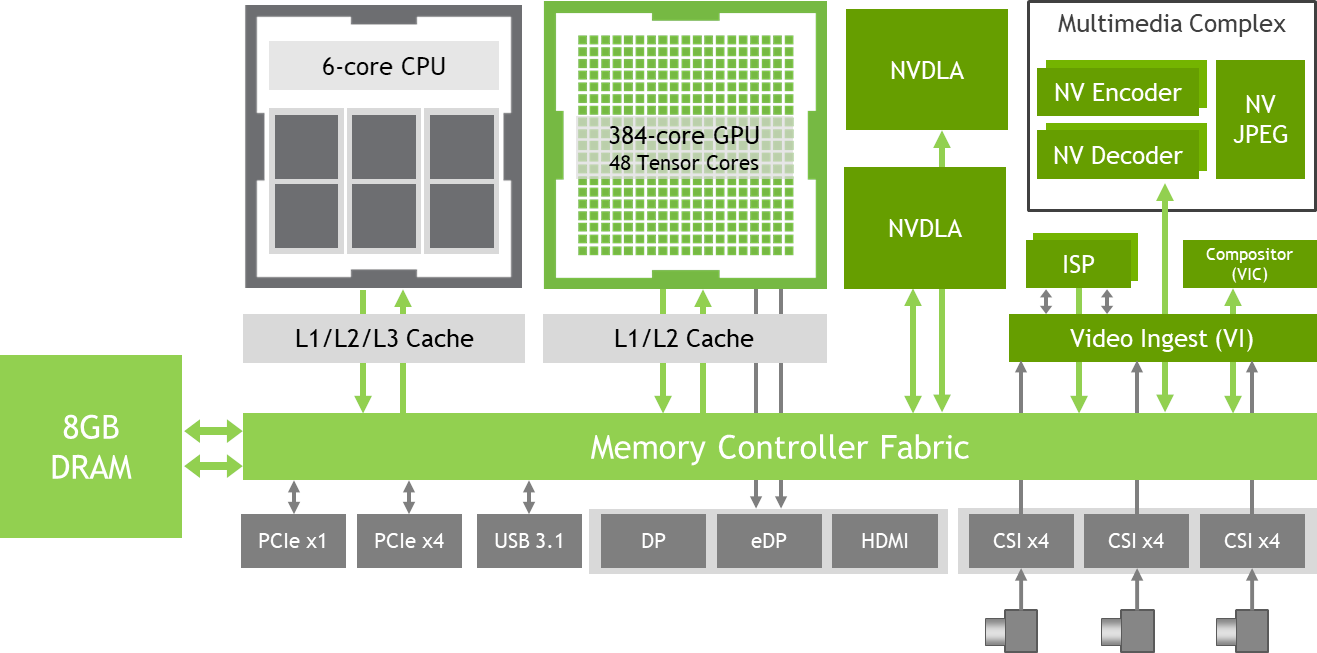
\includegraphics[width=0.90\textwidth]{images/Jetson_Xavier_NX_Block_Diagram.png}
    \caption{Block diagram of the technically equivalent Jetson Xavier NX. Note the shared DRAM and the separated caches for CPU and GPU. Copyright by Nvidia.}
    \label{im:XavierNX}
\end{figure}
\section{Software Architecture}
\label{sec:Software}
A single application needs to gather the data from the different sensors and cameras, apply the processing and render the result to an attached monitor. Within this application, various subsystems run in separate threads at different speeds. As visible in Figure \ref{fig:sw_concept}, the Vulkan framework, developed for a former thesis, is the skeleton of this application, to which additional C++ and CUDA modules got attached. Vulkan itself renders the 3D object – a rectangle named "projected image" – into the 2D viewfinder image of the main camera, as described in Section \ref{sec:VideoDisplay}. The image processing and the calculation of rotation and translation are mainly performed on the GPU, while the Kalman filtering is done on the CPU.\\
Due to the multithreaded nature of the system, and as multiple threads access the GPU simultaneously, the GPU access got grouped into different CUDA streams. \\
A separate application runs on the Raspberry Pi, serving a TCP/IP connection for streaming the ToF data. 
\begin{figure}[H]
    \centering
    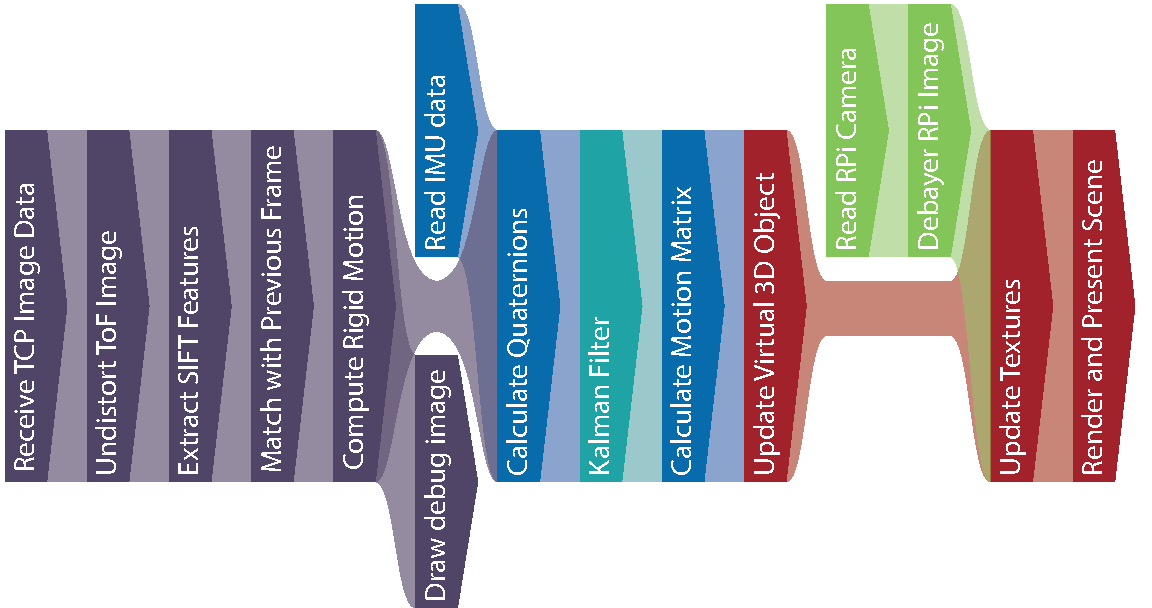
\includegraphics[width=0.75\textwidth]{images/data_flow.pdf}
    \caption{Data flow for one single frame. The colors are the same as in the software architecture overview in Figure \ref{fig:sw_concept}}
    \label{im:DataFlow}
\end{figure}

\begin{figure}[H]
    \centering
    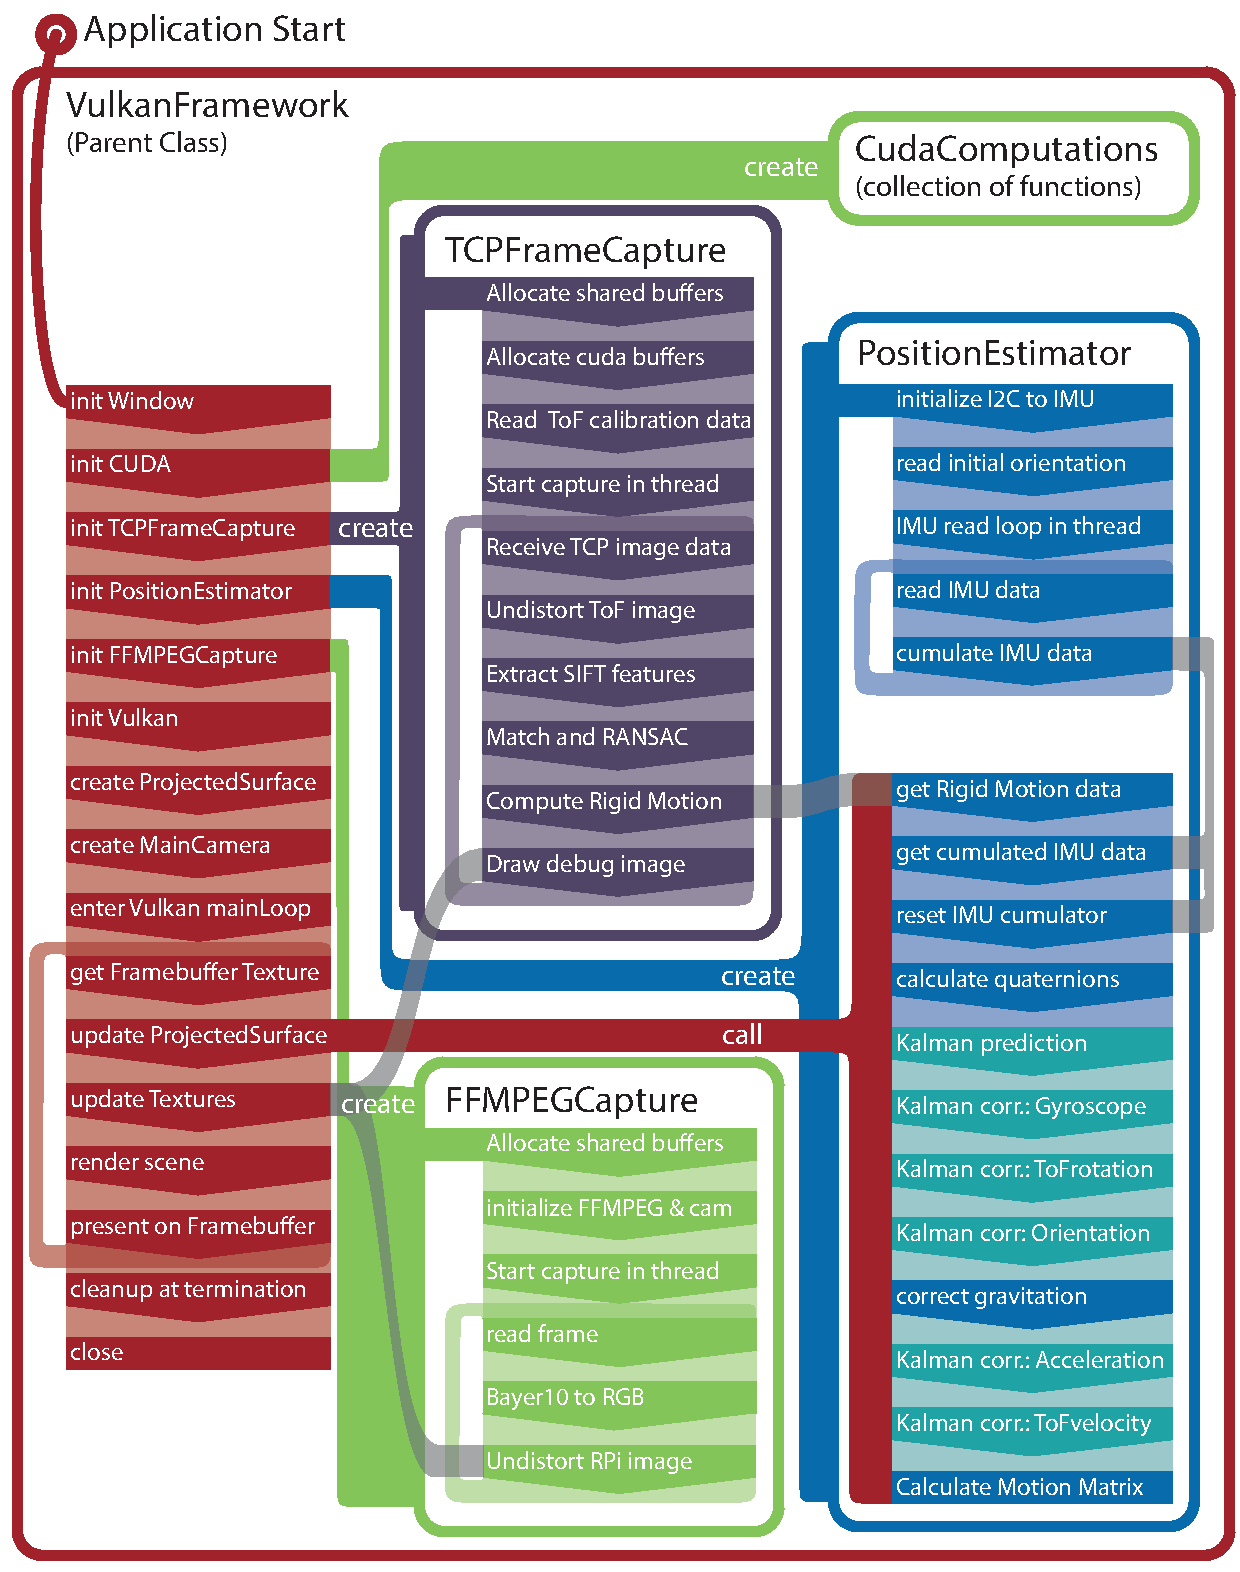
\includegraphics[width=1.0\textwidth]{images/SoftwareArchitecture.pdf}
    \caption{Software overview. The routine inside the Vulkan Framework creates four child classes.}
    \label{fig:sw_concept}
\end{figure}

\section{Motion estimation from ToF camera}
The following section describes the extraction of motion - rotational and translational velocity - from the ToF camera data. The purple section in Figure \ref{fig:sw_concept} shows the location of the algorithms within the software.
\subsection{ToF Camera calibration}
\label{sec:ToFCalibration}
On the ToF Camera, two parts need to be calibrated: The optics, as described in Section \ref{sec:FundCamCalibration}, and the distance measurement. The ToF camera has a barrel type distortion that is corrected by the camera calibration algorithm implemented in OpenCV\cite{openCVCamCalib} and shown in Figure \ref{fig.camCalib}. As the process of lens correction cuts off parts of the image, the image size gets reduced to 265 x 205 pixels.\\
For the distance measurement, first the radial distances need to be flattened as described in Section \ref{sec:ToFCamera}. As the angle $\alpha$ is not known for each pixel, a reference measurement is required. To reduce noise, 19 images of the same flat wall has been taken, smoothed by a two-dimensional gaussian filter and averaged onto one reference image $I_{Ref}$. The wireframe image in Figure \ref{im:ToFRaw} shows the curvature of this reference image. The rounding at the edges is an artifact of the gaussian smoothing.\\
\begin{figure}[H]
    \centering
    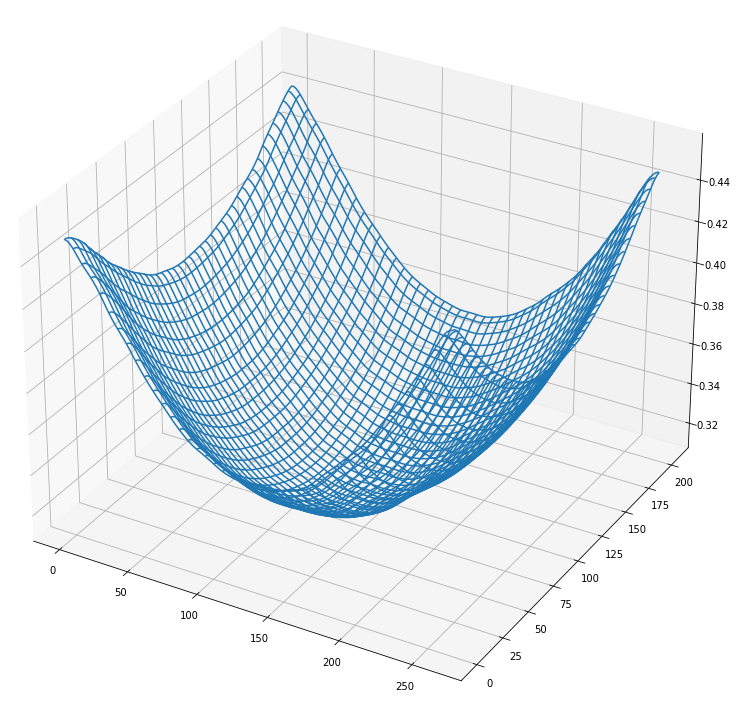
\includegraphics[width=0.4\textwidth]{images/raw_tof_radial.png}
    \caption{Wireframe rendering of the reference image $I_{Ref}$ provided by the ToF camera}
    \label{im:ToFRaw}
\end{figure}
Dividing the minimum value of this reference image $I_{Ref}$ with every pixel value generates a correcting map with $\cos \alpha$ values named
\begin{equation*}
    I_{cos} = \frac{\min (I_{Ref}) }{I_{Ref}}.
\end{equation*}
Pixel by pixel multiplication of any other image $I_{Any}$ with $I_{cos}$ will correct the influence of the radial measurement as shown in Figure \ref{im:ToFCorrected}. 
\begin{equation*}
    I_{Corr} = I_{cos}\cdot I_{Any}
\end{equation*}
\begin{figure}[H]
    \centering
    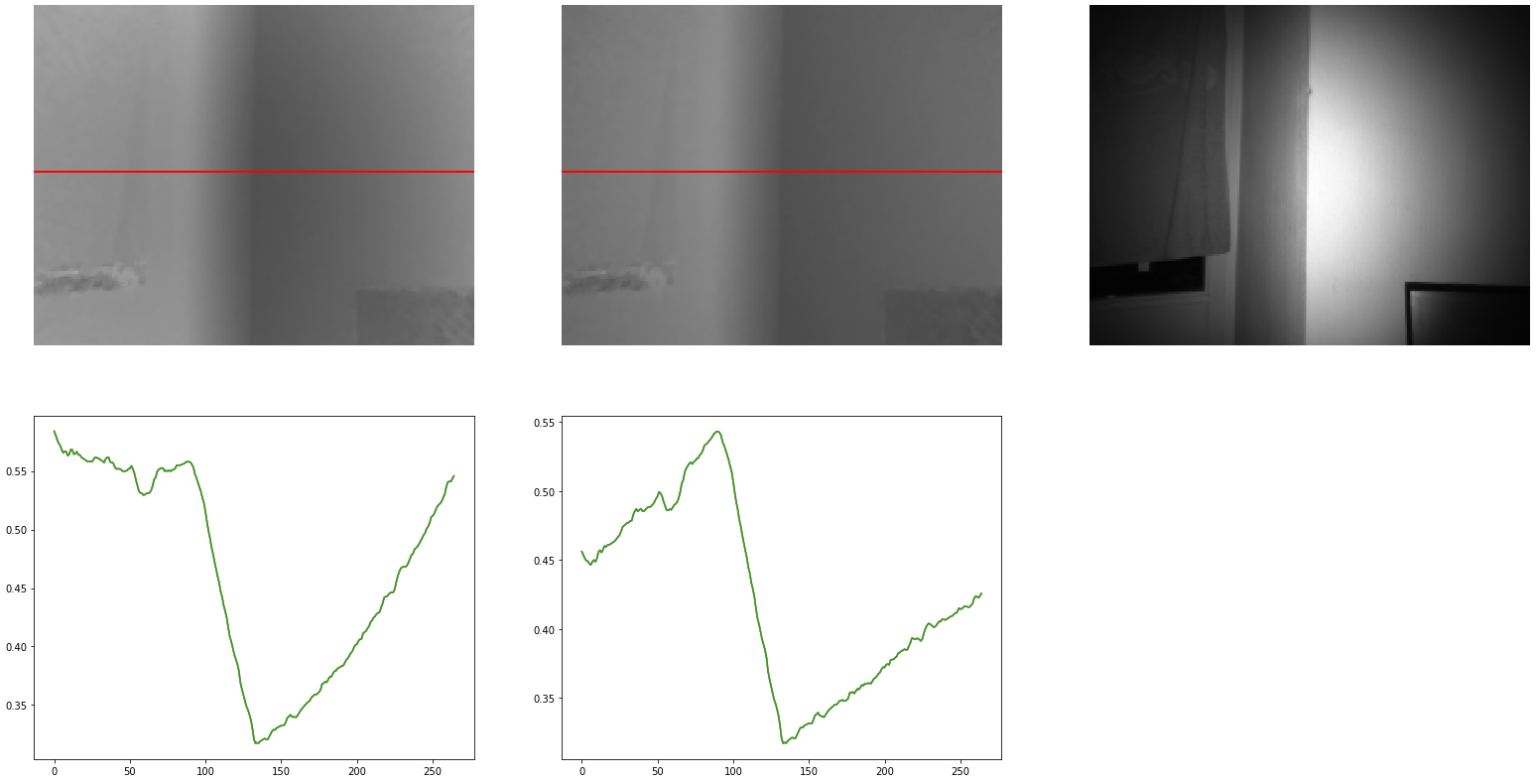
\includegraphics[width=1.0\textwidth]{images/flattened_tof_example.png}
    \caption{Left: uncorrected ToF image $I_{Any}$ Middle: the corrected image $I_{Corr}$ Right: the infrared grayscale image of the scene. To make the effect more apparent, the brightness accross the red lines have been plotted.}
    \label{im:ToFCorrected}
\end{figure}
To apply this calibration in CUDA, a file has been generated storing the $I_{Cos}$ values for each pixel in a lookup table. The application reads the file at initialization and keeps it stored in a Cuda allocated memory area. 

\subsection{SIFT feature extraction}
\label{sec:ToFPosition_SIFT}
The PiEye Nimbus ToF camera generates three different image channels for each picture: The depth map, the confidence, and the greyscale infrared image. By correcting the lens distortion as described in Section \ref{sec:FundCamCalibration}, straight lines in the real world get projected as straight lines on the images. By further correcting the characteristic of the ToF camera to measure radial distances, as described in Section \ref{sec:ToFCamera}, flat surfaces in the real world are also flat on the depth map. The implementations of both corrections are explained in Section \ref{sec:ToFCalibration}. \\
The points of the point clouds need to be matched to estimate rotation and translation between two consecutive ToF images. The CudaSift library\cite{cudaSiftRepo}\cite{CudaSiftPublication} extracts SIFT\cite{siftpaper} features on each greyscale infrared image of the ToF camera. Extraced features of the frame $k$, get brute-force matched with the features of the prior frame $k-1$, as visualized in Figure \ref{im:SiftExtraction}. SIFT features were chosen because of the author's prior experience, and it is a well-known feature extraction algorithm whose patent expired.\cite{siftpatent}
\begin{figure}[H]
    \centering
    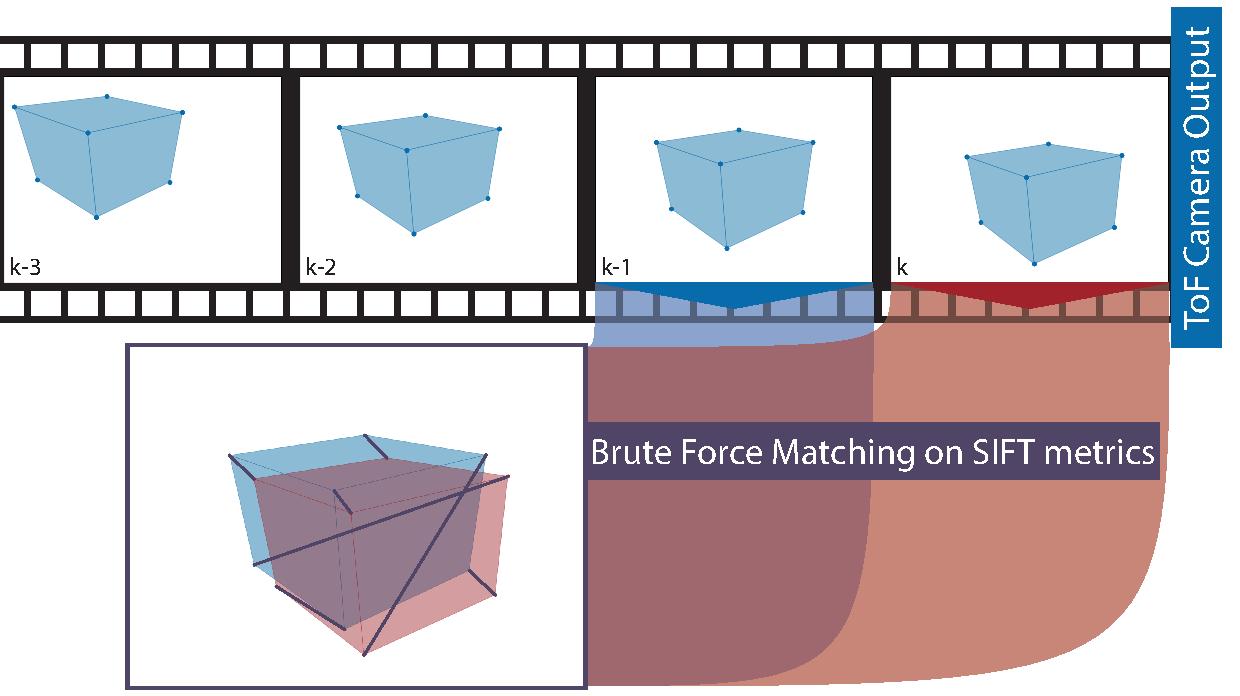
\includegraphics[width=1.0\textwidth]{images/feature_matching_bruteforce.pdf}
    \caption{First step of ToF motion estimation: Extract SIFT features and brute-force matching with prior image. Note that this brute-force matcher also generates false matches.}
    \label{im:SiftExtraction}
\end{figure}
Each feature coordinate on the picture gets mapped to the 3D space to generate a point cloud. The lens projects objects within the space of a pyramid onto the sensor, which leads to the following coordinate mapping. The coordinate transformation is visualized in Figure \ref{im:SiftCoordTransform}. Please note the coordinate convention described in Section \ref{sec:ABC_XYZ_coords}. The 3D coordinates $a$, $b$ and $c$ correspond to the image coordinates $u$ and $v$ via 
\begin{equation*}
    a = d \quad,\quad b = \frac{v}{f}\cdot x \quad,\quad c = \frac{u}{f}\cdot x.
\end{equation*}
$d$ is the value of the ToF depth image on position $(u,v)$. $f$ denotes a virtual focal length
\begin{equation*}
     f=\frac{\tfrac{u_{max}}{2}}{tan(\tfrac{\alpha}{2})},
\end{equation*}
merging the camera's field of view (viewing angle $\alpha$) and the image resolution in one number.
The PiEye Nimbus ToF camera has an advertised viewing angle of $1.152rad$ horizontally and $0.942rad$ vertically. Combined with an image resolution of $352 x 288px$. The results for $f$ for the horizontal case is $271$ and $282$ for the vertical case, thus value is set to $f = 280$.
\begin{figure}[H]
    \centering
    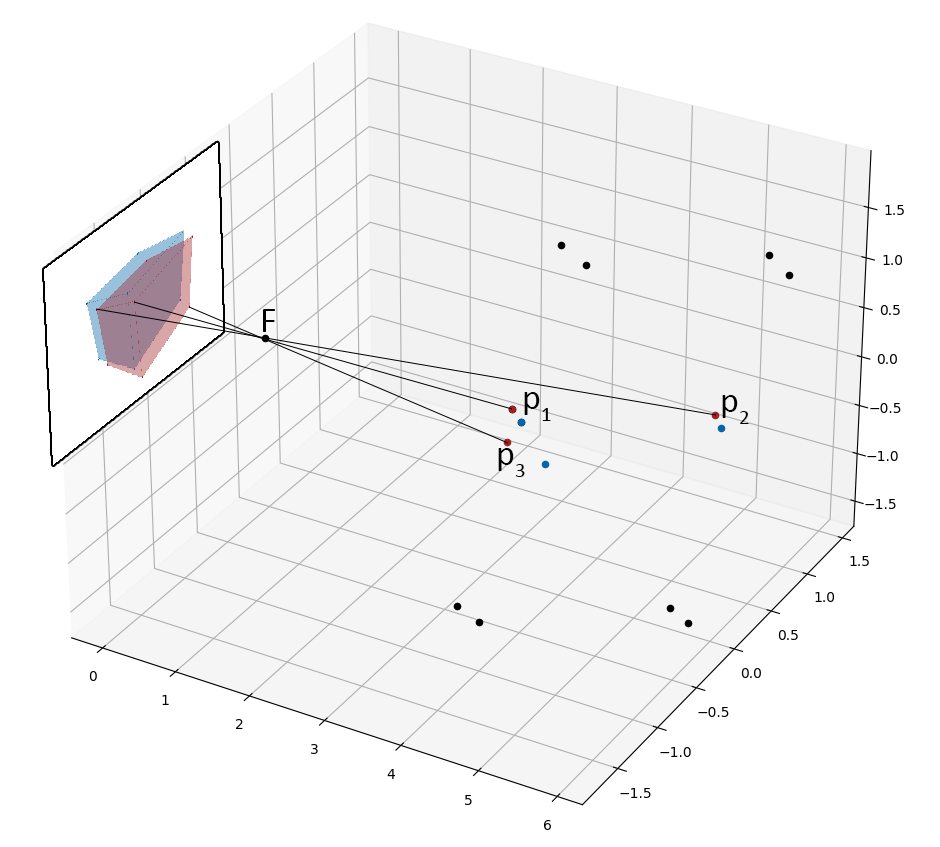
\includegraphics[width=1.0\textwidth]{images/2d_to_3d.png}
    \caption{Second step of ToF motion estimation: Map features into 3D space by setting }
    \label{im:SiftCoordTransform}
\end{figure}
\subsection{Estimation of rotation and translation}
\label{sec:ToFPosition_SVD}
Calculating the rotation and translation of one point cloud $P_{k-1}$ to another point cloud $P_{k}$ is possible with at least three correctly matched point pairs. Following the recipe from the ETH Zurich\cite{SVD_ETH}, also containing the proof, the three points must be centered.  Upper case $P$ denotes a point cloud, lower case $p$ denotes a single point in that cloud. The number of matched point pairs in the following formula is $n$, $i$ is the index of the single point in the point cloud and $k$ is the image frame number from which the point cloud got extracted.
The centroids for both point groups are:
\begin{equation*}
    \vec{c}_{k}=\frac{\sum_{i=1}^n \vec{p}_{i,k}}{n} \qquad 
    \vec{c}_{k-1}=\frac{\sum_{i=1}^n \vec{p}_{i,k-1}}{n} 
\end{equation*}
Subtraction of the centroid vectors from the individual points in the respective point cloud $P$ generates the centered point clouds $Q$. In an ideal case, a rotation matrix alone can transform one centered point cloud into the other. 
\begin{equation*}
    \vec{q}_{i,k}=\vec{p}_{i,k}-\vec{c}_{k} \qquad 
    \vec{q}_{i,k-1}=\vec{p}_{i,k-1}-\vec{c}_{k-1} \qquad i = 1, 2, 3, ... , n
\end{equation*}
Multiplying the transposed centered point group $Q_{k}$ with the point group $Q_{k-1}$ generates the $3\times3$ covariance matrix \begin{equation*}
    S= Q_{k-1}Q_{k}^{T}.
\end{equation*}
The point groups are packed in matrix form, each point being a column of the respective matrix. When using $n$ points, the point group matrices are of dimension $n\times3$, whose covariance matrix remains of dimension $3\times3$.\\
The singular value decomposition (SVD), explained in Section \ref{sec:SVD}, splits the covariance matrix $S$ into three separate $3\times3$ matrices $U$, $\Sigma$, and $V$. As the SVD in this use case is always applied to matrices of dimension $3\times3$, the optimized variant\cite{Gao:2018:GPU_MPM} from GitHub\cite{Github_SVD_CUDA} can be utilized.
\begin{equation*}
    S= U\Sigma V^{T}
\end{equation*}
The two rotation matrices $U$ and $V$ allow calculating the rotation between the point clouds\begin{equation*}
    R=V
    \begin{bmatrix}
        1 & 0 & 0 \\
        0 & 1 & 0 \\
        0 & 0 & det(VU^{T})
    \end{bmatrix}U^{T}.
\end{equation*}
Without the correction term $det(VU^{T})$ in the intermediate matrix, the method could generate a reflection instead of a rotation. This is numerically sound, but does not reflect the real world scenario. The determinant $det(VU^{T})$ equals -1 in the case of a reflection, which can be used to flip the signs of the 3rd column of the rotation matrix. If the SVD directly generates a rotation, $det(VU^{T})$ equals to 1, which transforms the intermediate matrix into the identity.\\
The wanted translation is computed by applying the rotation to the centroid vectors. 
\begin{equation*}
    \vec{t} = \vec{c}_{k}-R\cdot\vec{c}_{k-1}
\end{equation*}
The motion between the point clouds of consecutive the ToF images $k$ and $k-1$ is given by
\begin{equation*}
    \vec{p}_{i,k} = R\cdot\vec{p}_{i,k-1}+\vec{t}+E
\end{equation*}
with $R$ being the rotation matrix and $\vec{t}$ being the translation. For point clouds with $n=3$ the result is exact, for $n>3$, $E$ is the mean square error\cite{SVD_ETH}.
The estimated translation is only the translation between two frames. To estimate the velocity, the translation is divided by the sampling time.

\subsection{3D Random Sample Consensus (RANSAC)}
\label{sec:ToFPosition_RANSAC}
The motion estimation of the ToF camera relies on having good matches, which is not the case with the brute-force matcher, as the authors of the CudaSift library claim to have less than 50\% accuracy on its brute-force matcher.\cite{cudaSiftRepo} Low matching accuracy is a known problem in other fields of image processing - like panorama stitching - and is there often solved with an algorithm named RANSAC (random sample consensus).\\
These applications of the RANSAC algorithm work on two-dimensional images and are not suitable for three-dimensional point clouds; therefore, an extension to the RANSAC algorihm is proposed in the following.\\
The first step of the three-dimensional RANSAC is finding a proper rotation and translation from the brute-force matches. To find these transformations, each matched feature pair gets two other feature pairs randomly assigned. To each group of three feature pairs, the rotation and translation is calculated using the method described in Section \ref{sec:ToFPosition_SVD} as shown in Figure \ref{im:ransac1}.
\begin{figure}[H]
    \centering
    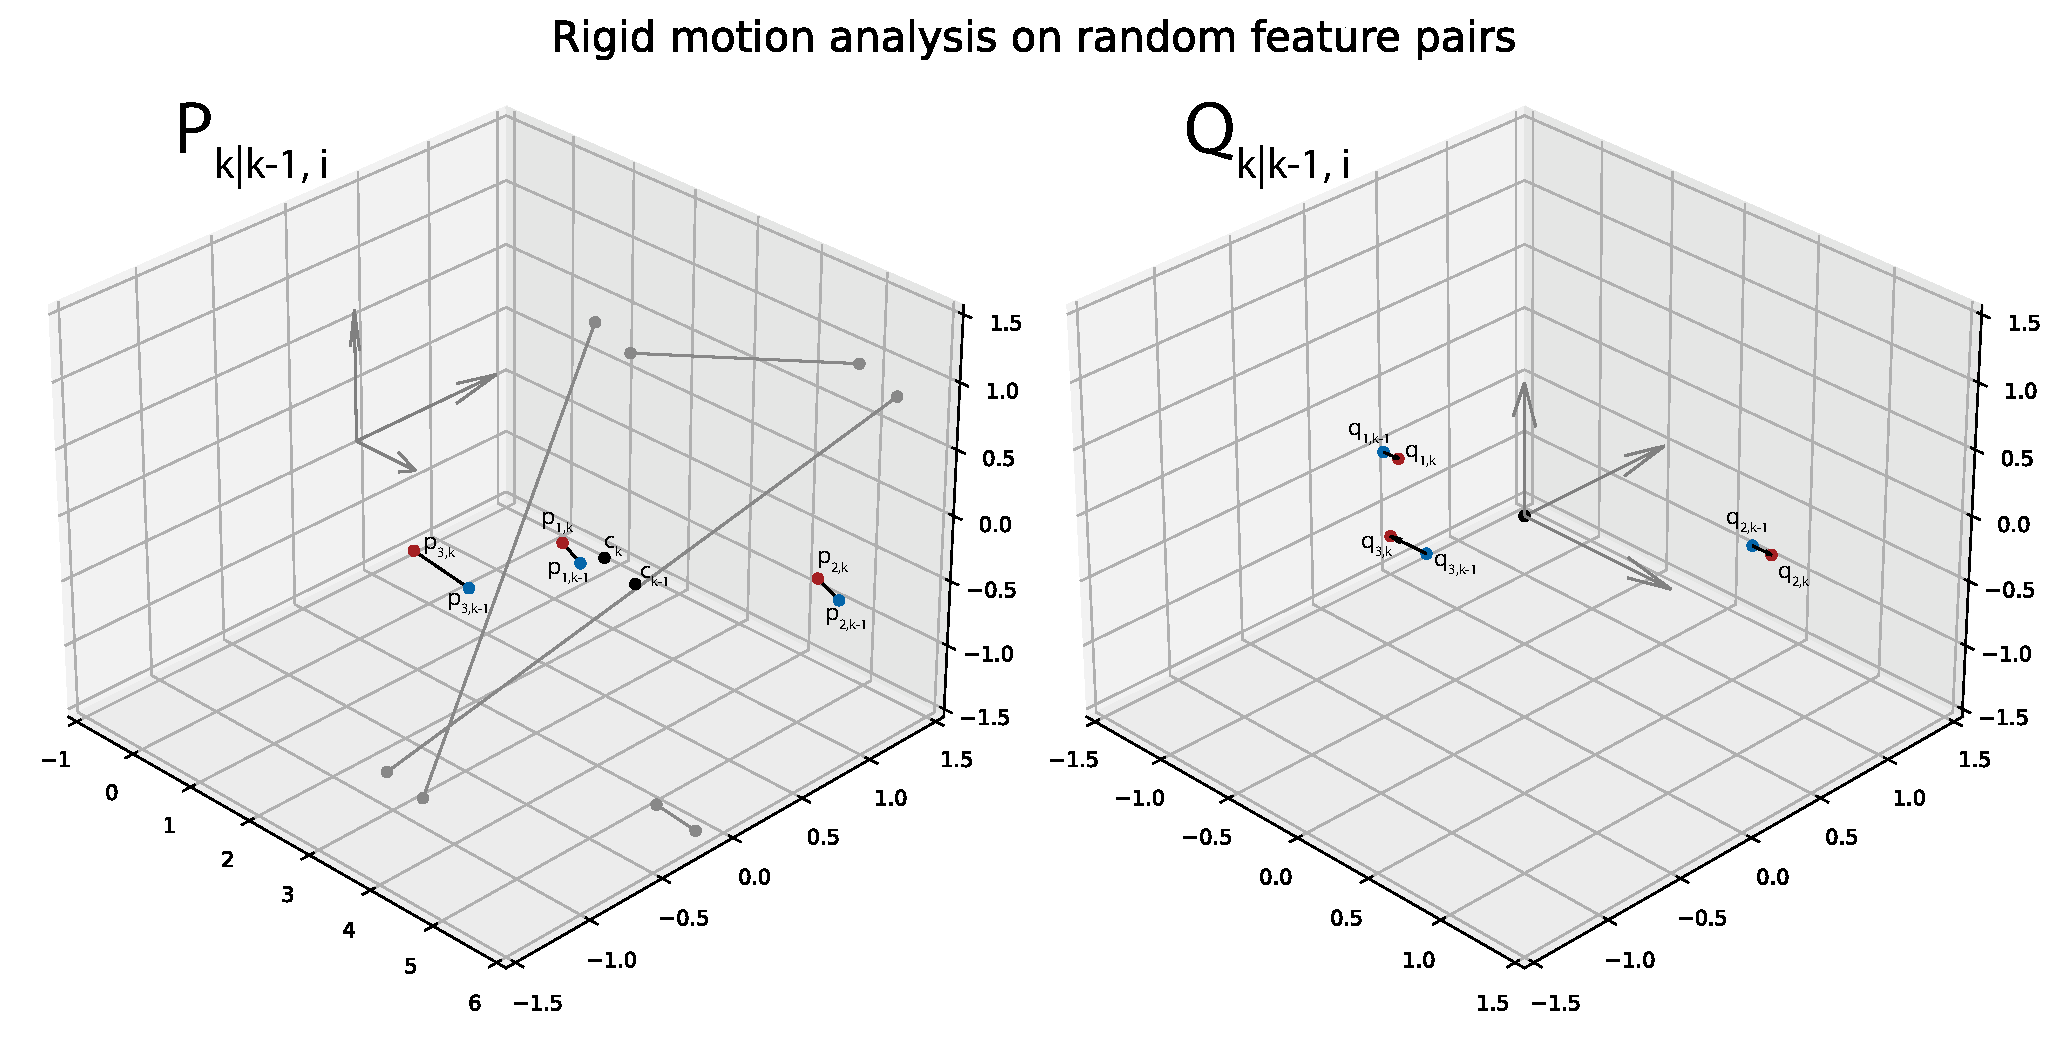
\includegraphics[width=0.95\textwidth]{images/ransac_3d_step1.pdf}
    \caption{First step of the 3D RANSAC: Using the SVD method for estimating the rotation and translation from three randomly assigned points. This step is performed in parallel on multiple groups of three. Each group $P_{i}$ generates the rotation $R_{i}$ and translation $\vec{t}_{i}$.}
    \label{im:ransac1}
\end{figure}
Each group's calculated rotation matrices and translation vectors get checked against all the other matched feature pairs. The data point from the previous image of the feature pair gets transformed by the matrix-vector-pair and compared to the data point of the current picture. If the sum of square differences (SSD) of the two points is lower than a threshold, the feature pair is marked as a proper motion, as shown in Figure \ref{im:ransac2}. Over all these proper points, the average distance is calculated for each group of three feature pairs. The estimated matrix-vector-pair that generates the smallest average distance is likely suitable for further processing.
\begin{figure}[H]
    \centering
    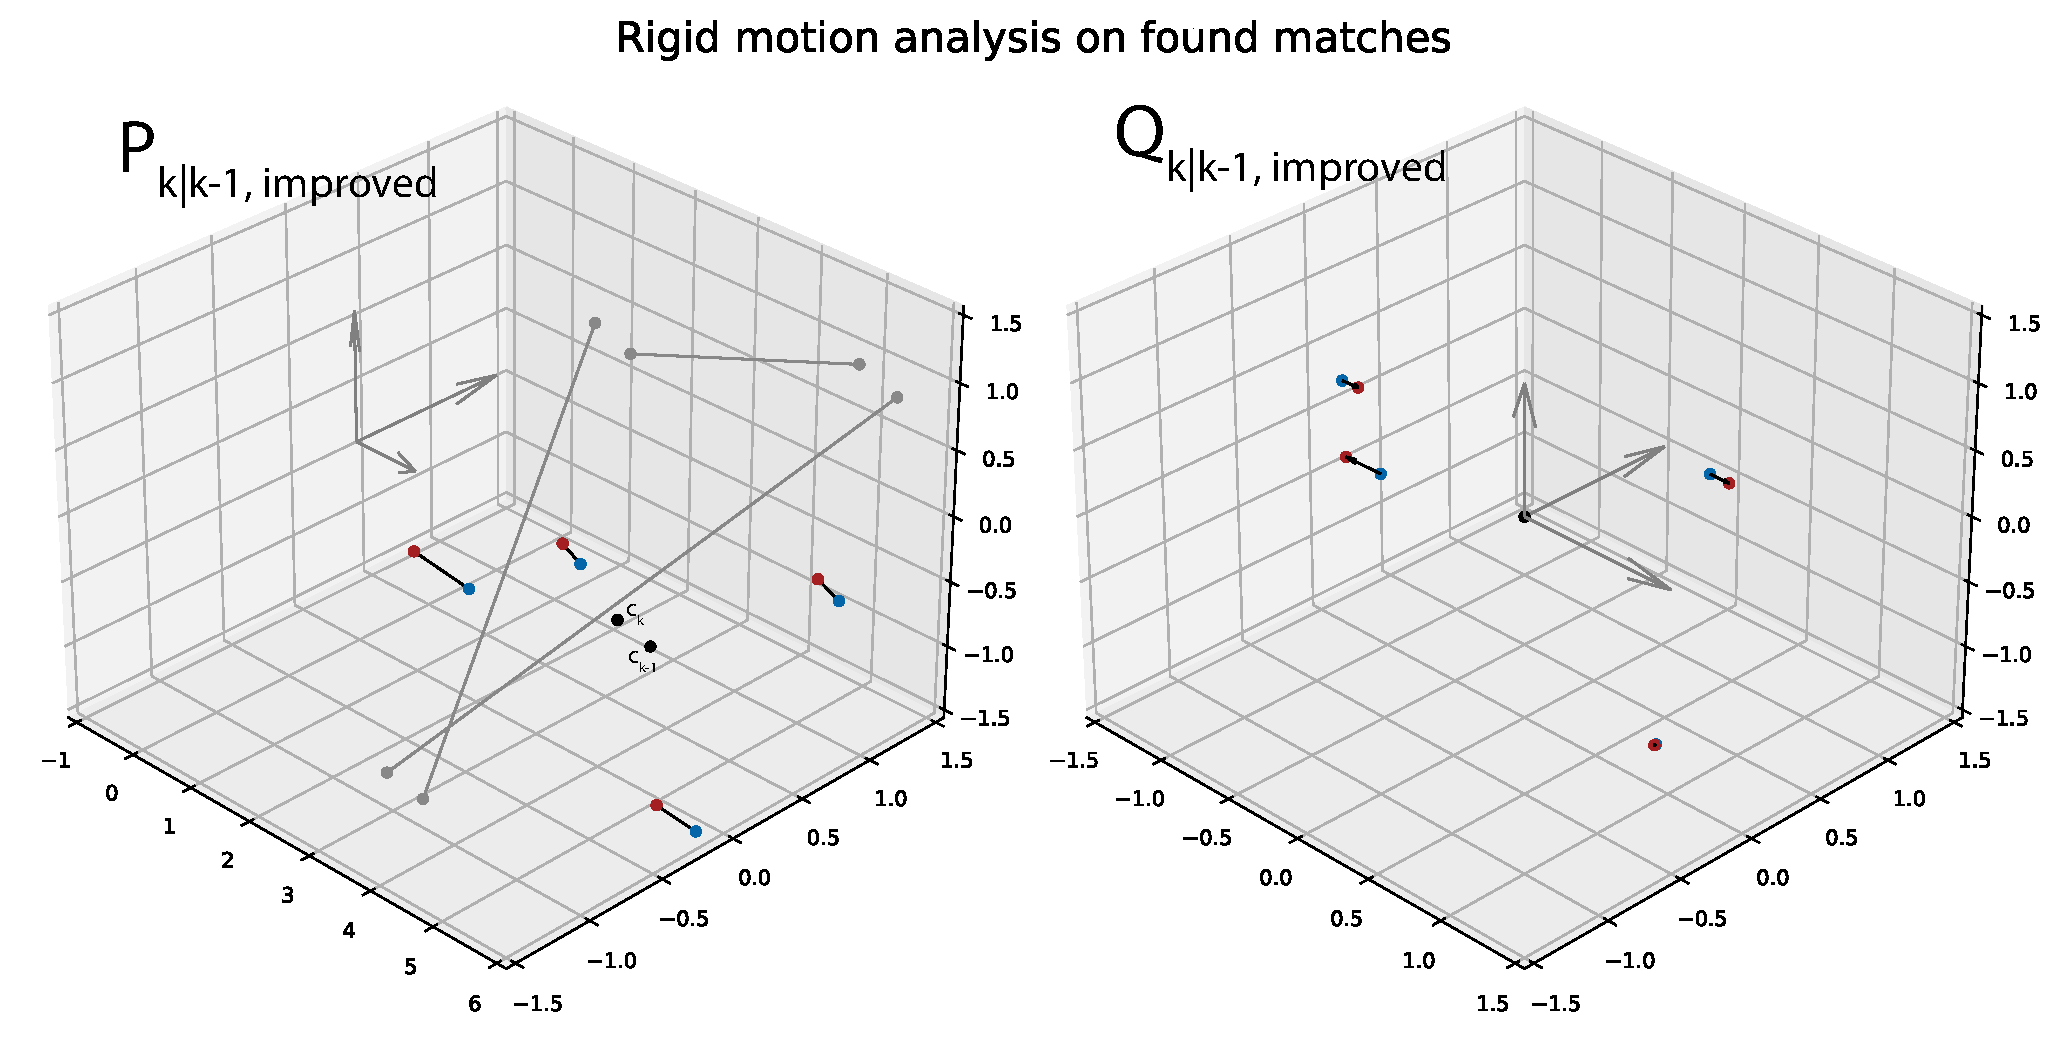
\includegraphics[width=0.95\textwidth]{images/ransac_3d_step2.pdf}
    \caption{Second step of the 3D RANSAC: The calculated rotations and translations get evaluated against the whole dataset. In the example, the fourth matching point fulfills the criterion.}
    \label{im:ransac2}
\end{figure}
 In a third step, applying the SVD method to all the proper feature pairs as larger point clouds generates the improved motion $R_{improved}$ and $\vec{t}_{improved}$. \\
Ignoring the SIFT metrics that lead to the brute force matching, all the features get matched again based on the position alone, using the rotation $R_{improved}$ and translation $\vec{t}_{improved}$ estimated before. The matrix-vector pair transforms every data point from the previous image. The distance between the transformed point and the closest data point of the current picture determines the new match. If the proximity is below a threshold, the match is marked for the last step.
\begin{figure}[H]
    \centering
    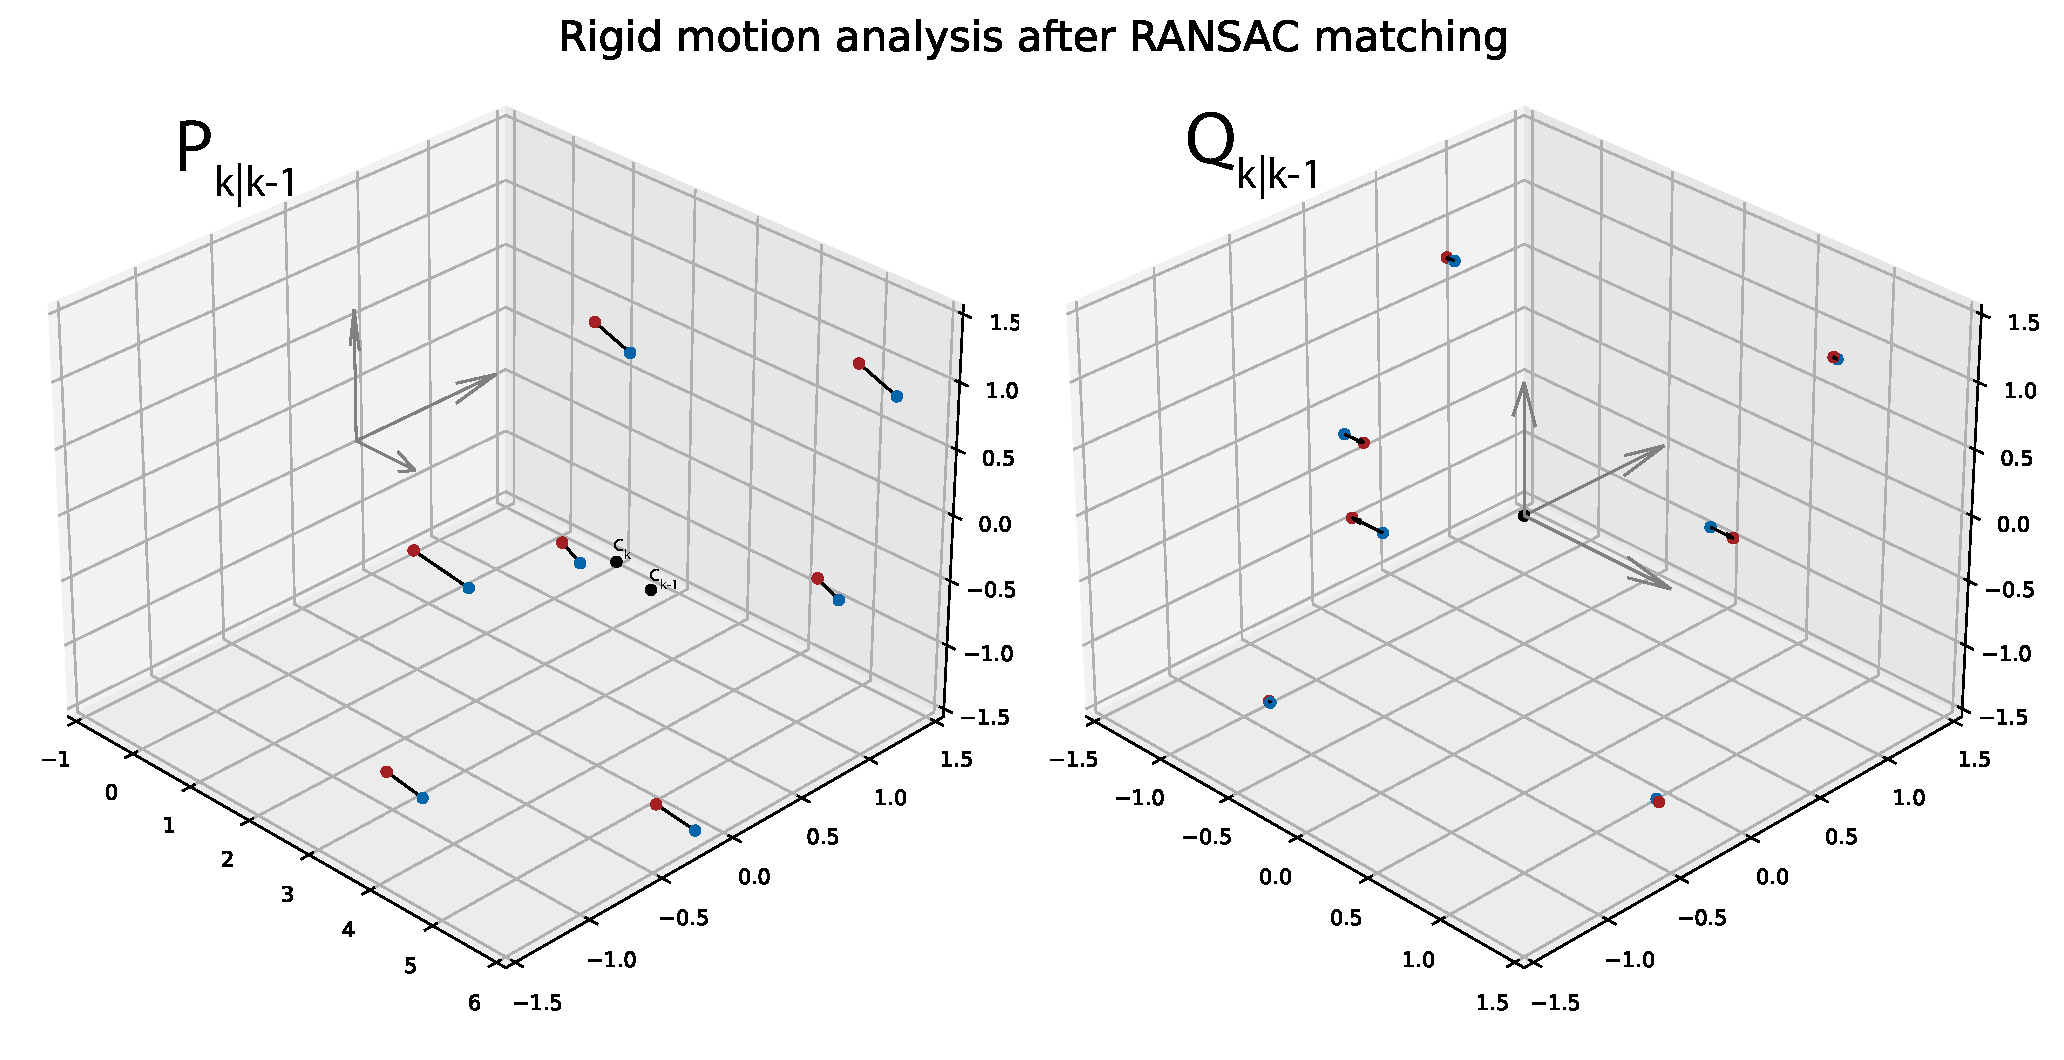
\includegraphics[width=0.95\textwidth]{images/ransac_3d_step3.pdf}
    \caption{Third step of the 3D RANSAC: Applying the currently available rotation- and translation-information the the point clouds allows re-matching based alone on the position. The optimal rotation $R_{opt}$ and translation $\vec{t}_{opt}$ result from these feature pairs.}
    \label{im:ransac3}
\end{figure}
Finally, the optimal rotation matrix $R_{opt}$ and translation vector $\vec{t}_{opt}$ are estimated using the same SVD method, using all RANSAC matches.
\section{Sensor Fusion}
\label{sec:PositionEstimate}
The following section describes the implementation of the accelerometer and gyroscope processing, marked blue in Figure \ref{fig:sw_concept}, and the Kalman filter, marked in cyan in the same image, which fuses the data with the ToF camera motion data.

\subsection{Gyroscope and Accelerometer}
\label{sec:GyroCal}
The 6-axis IMU Bosch BMI160 provides gyroscope and accelerometer measurements via an I²C connection, extended by a Silicon Labs CP2112 USB-to-I²C bridge. The BMI160 is soldered onto a module by DFRobot. The IMU generates measurements regarding acceleration in the directions $a$, $b$, and $c$, and measurements regarding rotation speed around these axes.\\
As the gyroscope and accelerometer output incremental movement, the values need to be integrated over time. Accurate data is crucial compensate for gravity or for detecting movement - especially because of positional information being the result of integrating the acceleration twice.\\
The range of the acclerometer is variable and has been set to ±8 G, it has an output resolution of 16 bit and an output data rate of 200 Hz.
The accelerometer was calibrated in 24 orientations to compensate for angular errors in the IMU, on the PCB and of the calibration table. For each orientation, 100 raw measurements have been averaged to eliminate noise. 
The largest error has been 38 mG, that lies within the sensor's specification of ±40 mG\cite{BMI160}. In addition, the gain for the accelerometer has been corrected based on gravity. A maximum error of 1.8\% has been measured and corrected, which also is in the sensor's specification of ±0.5\% full scale\cite{BMI160}.\\
For the gyroscope, the range is set to ±2000 degrees per second with an output data rate of 200 Hz. The gyroscope has been calibrated only for zero offset, whose maximum error was 0.2 degrees per second which is well in the specified ±3 degrees per second\cite{BMI160}.\\
The IMU shows a hysteresis that is within the specification of the datasheet; therefore, a simple offset correction does not yield the best results. A moving average – that gets updated whenever no motion of the camera head is detected – helps deal with the hysteresis by subtraction from the measurement value.

\section{Sensor Fusion with Kalman Filter}
\label{sec:SensorFusion}
The combination of data coming from different sensors or sensor types is named sensor fusion. In this case, the accelerometer and the calculated motion from the ToF camera add information to the system describing the same movement. Both sensors have noise and inaccuracies that need to be considered to calculate the system state $\vec{x}$, which includes the current position, velocity, acceleration, angular orientation, and angular velocity.\\
A Kalman filter, explained in Section \ref{sec:Kalmanfilter}, fuses the motion information of the ToF camera with the measurements from the IMU. The system requires equal sampling rates for the individual sensors. Therefore, the IMU data is downsampled to match the ToF camera's framerate.
With the translational information being present in all three directions and the rotation being inserted in quaternion form, the system state vector is
\begin{equation*}
    \vec{x}^{T} = (
        x, \dot{x}, \ddot{x}, y, \dot{y}, \ddot{y}, z, \dot{z}, \ddot{z}, r_{a}, r_{b}, r_{c}, r_{d}, \dot{r}_{a}, \dot{r}_{b}, \dot{r}_{c}, \dot{r}_{d}).
\end{equation*}
$x$, $y$ and $z$ describe the position in space, and $r_{a}$, $r_{b}$, $r_{c}$, and $r_{d}$ being the components of the orientation quaternion $R = (a, b\textbf{i}, c\textbf{j}, d\textbf{k})$. The time-derivatives of these values are denoted with overdots.
\begin{equation*}
    \vec{x}^{T} = (
        x, \dot{x}, \ddot{x}, y, \dot{y}, \ddot{y}, z, \dot{z}, \ddot{z}, r_{a}, r_{b}, r_{c}, r_{d}, \dot{r}_{a}, \dot{r}_{b}, \dot{r}_{c}, \dot{r}_{d})
\end{equation*}
\subsection{Prediction}
\label{sec:KalmanPrediction}
The model matrix $F$ describes the evolution of the system state $\vec{x}$ via \begin{equation*}
    \vec{x}_{k|k-1} = 
    F
    \cdot
    \vec{x}_{k-1}.
\end{equation*} 
The velocities and accelerations both alter the position, while the accelerations alter the velocities. For the rotation, the quaternion containing the angular rotation already contains the sampling rate and gets added by a quaternion multiplication. 

The $\dot{r}$-values in the matrix are from $\vec{x}_{k-1}$ and $\Delta t$ is the sampling rate.
\begin{equation*}
    \begin{pmatrix}
        x_{k|k-1}\\
        \dot{x}_{k|k-1}\\
        \ddot{x}_{k|k-1}\\
        y_{k|k-1}\\
        \dot{y}_{k|k-1}\\
        \ddot{y}_{k|k-1}\\
        z_{k|k-1}\\
        \dot{z}_{k|k-1}\\
        \ddot{z}_{k|k-1}\\
        r_{a,k|k-1}\\
        r_{b,k|k-1}\\
        r_{c,k|k-1}\\
        r_{d,k|k-1}\\
        \dot{r}_{a,k|k-1}\\
        \dot{r}_{b,k|k-1}\\
        \dot{r}_{c,k|k-1}\\
        \dot{r}_{d,k|k-1}
    \end{pmatrix} = 
    \begin{bmatrix}
        1 & \Delta t & \frac{\Delta t^{2}}{2} &  &  &  &  &  &  &  &  &  & & &  &  &  \\
        0 & 1 & \Delta t & &  &  &  &  &  &  &  & \cdot &  &  &  &  &  \\
        0 & 0 & 1 &  &  &  &  &  &  &  &  & \cdot &  &  &  &  &  \\
         &  &  & 1 & \Delta t & \frac{\Delta t^{2}}{2} &  &  &  & \cdot & \cdot & 0 & \cdot & \cdot &  &  &  \\
         &  &  & 0 & 1 & \Delta t &  &  &  &  &  & \cdot &  &  &  & &  \\
         &  &  & 0 & 0 & 1 &  &  &  &  &  & \cdot &  &  &  &  &  \\
         &  &  &  &  &  & 1 & \Delta t & \frac{\Delta t^{2}}{2} &  &  &  &  &  &  &  &  \\
         &  &  &  &  &  & 0 & 1 & \Delta t &  &  &  &  &  &  &  &  \\
         &  &  &  &  &  & 0 & 0 & 1 &  &  &  &  &  &  &  &  \\
         &  &  & \cdot &  &  &  &  &  & \dot{r}_{a} & -\dot{r}_{b} & -\dot{r}_{c} & -\dot{r}_{d} &  &  &  &  \\
         &  &  & \cdot &  &  &  &  &  & \dot{r}_{b} &  \dot{r}_{a} &  \dot{r}_{d} & -\dot{r}_{c} &  &  &  &  \\
         & \cdot & \cdot & 0 & \cdot & \cdot &  &  &  & \dot{r}_{c} & -\dot{r}_{d} &  \dot{r}_{a} &  \dot{r}_{b} &  &  &  &  \\
         &  &  & \cdot &  &  &  &  &  & \dot{r}_{d} &  \dot{r}_{c} & -\dot{r}_{b} &  \dot{r}_{a} &  &  &  &  \\
         &  &  & \cdot &  &  &  &  &  &  &  &  &  & 1 & 0 & 0 & 0 \\
         &  &  &  &  &  &  &  &  &  &  &  &  & 0 & 1 & 0 & 0 \\
         &  &  &  &  &  &  &  &  &  &  &  &  & 0 & 0 & 1 & 0 \\
         &  &  &  &  &  &  &  &  &  &  &  &  & 0 & 0 & 0 & 1
    \end{bmatrix} 
    \cdot 
    \begin{pmatrix}
        x_{k-1}\\
        \dot{x}_{k-1}\\
        \ddot{x}_{k-1}\\
        y_{k-1}\\
        \dot{y}_{k-1}\\
        \ddot{y}_{k-1}\\
        z_{k-1}\\
        \dot{z}_{k-1}\\
        \ddot{z}_{k-1}\\
        r_{a,k-1}\\
        r_{b,k-1}\\
        r_{c,k-1}\\
        r_{d,k-1}\\
        \dot{r}_{a,k-1}\\
        \dot{r}_{b,k-1}\\
        \dot{r}_{c,k-1}\\
        \dot{r}_{d,k-1}
    \end{pmatrix}
\end{equation*}
The $\dot{r}$ values inside the model matrix $F$ are the same as in the vector $\vec{x}_{k-1}$. Technically, the operation is not a linear transformation anymore, as the quaternion multiplication itself is not linear.\\
The second step of the prediction is the prediction of the covariance matrix of the errors $P$. 
\begin{equation*}
    P_{k|k-1} = 
    F
    \cdot
    P_{k-1}
    \cdot
    F^{T}
    +
    N
\end{equation*}
The Kalman filter relies on knowing the uncertainties of the model. If a system has rigid constraints by design, the sensor data will naturally be interpreted to support the model. The model of the camera head has loose restrictions, as the camera head is free to move in any direction and rotation; therefore, the output heavily relies on the sensor data.\\
While $P_{0}$ starts as identity matrix, $N$ is the gaussian process noise, see Section \ref{sec:Kalmanfilter} for the translational part. For the rotation, the diagonal elements got set to 50, making the system noise vastly bigger than the noise of the input data.\\
Generally, a large process noise leads to a lower emphasis to the current system state and larger weight to the sensor data.\\ 
\begin{equation*}
    N = 
    \begin{bmatrix}
        \frac{\Delta t^{4}}{4} & \frac{\Delta t^{3}}{2} & \frac{\Delta t^{2}}{2} &  &  &  &  &  &  &  &  &  & & &  &  &  \\
        \frac{\Delta t^{3}}{2} & \Delta t^{2} & \Delta t  & &  &  &  &  &  &  &  & \cdot &  &  &  &  &  \\
        \frac{\Delta t^{2}}{2} & \Delta t & 1 &  &  &  &  &  &  &  &  & \cdot &  &  &  &  &  \\
         &  &  &  \frac{\Delta t^{4}}{4} & \frac{\Delta t^{3}}{2} & \frac{\Delta t^{2}}{2}  &  &  &  & \cdot & \cdot & 0 & \cdot & \cdot &  &  &  \\
         &  &  &  \frac{\Delta t^{3}}{2} & \Delta t^{2} & \Delta t &  &  &  &  &  & \cdot &  &  &  & &  \\
         &  &  &  \frac{\Delta t^{2}}{2} & \Delta t & 1 &  &  &  &  &  & \cdot &  &  &  &  &  \\
         &  &  &  &  &  &  \frac{\Delta t^{4}}{4} & \frac{\Delta t^{3}}{2} & \frac{\Delta t^{2}}{2} &  &  &  &  &  &  &  &  \\
         &  &  &  &  &  &  \frac{\Delta t^{3}}{2} & \Delta t^{2} & \Delta t &  &  &  &  &  &  &  &  \\
         &  &  &  &  &  &  \frac{\Delta t^{2}}{2} & \Delta t & 1 &  &  &  &  &  &  &  &  \\
         &  &  & \cdot &  &  &  &  &  & 1 & 0 & 0 & 0 &  &  &  &  \\
         &  &  & \cdot &  &  &  &  &  & 0 & 1 & 0 & 0 & &  &  &  \\
         & \cdot & \cdot & 0 & \cdot & \cdot &  &  &  & 0 & 0 & 1 & 0 &  & &  &  \\
         &  &  & \cdot &  &  &  &  &  & 0 & 0 & 0 &  1 &  &  &  &  \\
         &  &  & \cdot &  &  &  &  &  &  &  &  &  & 50 & 0 & 0 & 0 \\
         &  &  &  &  &  &  &  &  &  &  &  &  & 0 & 50 & 0 & 0 \\
         &  &  &  &  &  &  &  &  &  &  &  &  & 0 & 0 & 50 & 0 \\
         &  &  &  &  &  &  &  &  &  &  &  &  & 0 & 0 & 0 & 50
    \end{bmatrix}
\end{equation*}
\subsection{Correction: Rotation}
\label{sec:CorrectionRotation}
The Kalman filter allows chaining multiple correction steps after another, which helps add data of different sensors to the same input and helps simplify the calculation. The observation matrix H maps the four quaternion values of an input – gyroscope or ToF camera – to the 17 values of the system state vector x. Choosing a $4\times17$ matrix changes the bracket of the following equation to a $4\times4$ matrix, simplifying the matrix inversion for calculating the Kalman gain. The iteration $n$ in the equations denote the number of the chained correction steps, as the system state vector $\vec{x}$ and the covariance matrix of errors $P$ are updated in each step.
\begin{equation*}
    K_{k|k-1|n} = P_{k|k-1|n}\cdot H^{T}(H\cdot P_{k|k-1|n}\cdot H^{T}+R)^{-1}
\end{equation*}
The order of the subsequent correction steps is irrelevant. The following H maps the rotation speed to the system state and is used for both sensors.
\begin{equation*}
    H=
    \begin{bmatrix}
        0 & 0 & 0 & 0 & 0 & 0 & 0 & 0 & 0 & 0 & 0 & 0 & 0 & \textbf{1} & 0 & 0 & 0 \\
        0 & 0 & 0 & 0 & 0 & 0 & 0 & 0 & 0 & 0 & 0 & 0 & 0 & 0 & \textbf{1} & 0 & 0 \\
        0 & 0 & 0 & 0 & 0 & 0 & 0 & 0 & 0 & 0 & 0 & 0 & 0 & 0 & 0 & \textbf{1} & 0 \\
        0 & 0 & 0 & 0 & 0 & 0 & 0 & 0 & 0 & 0 & 0 & 0 & 0 & 0 & 0 & 0 & \textbf{1}
    \end{bmatrix}
\end{equation*}
For both sensors – the gyroscope and the ToF camera – R is a diagonal matrix with the standard deviation of the respective sensor as its values.
\begin{equation*}
    R = \sigma \cdot I
\end{equation*}
The rotation quaternion $Q_{Rot}=(r_{c}, a_{c}\textbf{i}, b_{c}\textbf{j}, c_{c}\textbf{k})$ represents the new observation $\vec{z}_{k} = r_{c}, a_{c}, b_{c}, c_{c}$. With the following equations, the system state vector and the covariance matrix of the errors get calculated for the next iteration.
\begin{equation*}
    x_{k} = \vec{x}_{k|k-1|n}+K_{k}(\vec{z}_{k}-H\cdot \vec{x}_{k|k-1|n})
    \qquad ; \qquad
    P_{k|k-1|n+1}= (I-K_{k}\cdot H)P_{k|k-1|n}
\end{equation*}
The quaternion multiplication inside the model matrix $F$ adds up the subsequent rotation speed in each iteration to the cumulated rotation. The Kalman correction step for rotations is carried out for the data of the ToF camera and the data of the Gyroscope, one after another.

\subsection{Rotation Drift compensation with Accelerometer}
\label{sec:RotDriftCompensation}
When the camera head is stationary, the accelerometer measures the direction of gravity, allowing the correction of rotation on the x- and y-axis.  Using the earth's magnetic field, a magnetometer could compensate for the drift on the z-axis, but the used IMU does not contain one.
Knowing the system's orientation quaternion at the start $Q_{init}$ of the application and the cumulated rotation $R$, calculating the system's current orientation $Q_{c}$ is a quaternion multiplication, as described in Section \ref{sec:RotationQuaternion}. If the orientation drifted, it would be different from the measured orientation $Q_{m}$ derived from the accelerometer. The complex parts of the two orientation quaternions get normalized and stored in individual vectors $\vec{s}$ and $\vec{d}$. 
\begin{equation*}
    Q_{c} =
    \begin{pmatrix}
        r_{c}           \\
        a_{c}\textbf{i} \\
        b_{c}\textbf{j} \\
        c_{c}\textbf{k}
    \end{pmatrix} \quad ; \quad
    \vec{v}_{c} =
    \begin{pmatrix}
        a_{c} \\
        b_{c} \\
        c_{c}
    \end{pmatrix} 
    \quad ; \quad
    \vec{s} = \frac{\vec{v}_{c}}{|\vec{v}_{c}|} 
    \quad ; \quad
    Q_{m} =
    \begin{pmatrix}
        r_{m}           \\
        a_{m}\textbf{i} \\
        b_{m}\textbf{j} \\
        c_{m}\textbf{k}
    \end{pmatrix} \quad ; \quad
    \vec{v}_{m} =
    \begin{pmatrix}
        a_{m} \\
        b_{m} \\
        c_{m}
    \end{pmatrix} 
    \quad ; \quad
    \vec{d} = \frac{\vec{v}_{m}}{|\vec{v}_{m}|}          
\end{equation*}
The dot product of the two normalized vectors calculates the cosine of the angle between the vectors $\theta$, and the cross product calculates the rotation axis $\vec{r}$. 
\begin{equation*}
    cos(\theta) = \vec{s}\cdot\vec{d} \quad ; \quad \vec{r} = \vec{s}\times\vec{d} \quad ; \quad
    \vec{r} =
    \begin{pmatrix}
        r_{1} \\
        r_{2} \\
        r_{3}
    \end{pmatrix} 
\end{equation*}
Estimating the value $x$ from the angle helps scale the values for generating a correcting rotation quaternion $Q_{corr}$.
\begin{equation*}
    x=\sqrt{(1+cos(\theta)*2)} \quad ; \quad Q_{corr} =
    \begin{pmatrix}
        0.5\cdot x           \\
        r_{1}\cdot\frac{1}{x}\textbf{i} \\
        r_{2}\cdot\frac{1}{x}\textbf{j} \\
        r_{3}\cdot\frac{1}{x}\textbf{k}
    \end{pmatrix}    
\end{equation*}
An additional Kalman correction step adds the correcting rotation quaternion $Q_{corr}$ to the system. The calculation is the same as for the rotation quaternions from the gyroscope and the ToF camera, which is described in Section \ref{sec:CorrectionRotation}.
\subsection{Correction: Translation}
Data from the accelerometer and the translational velocity from the ToF camera get sampled in $a$, $b$ and $c$ coordinates, as the sensors rotate with the whole camera head. The speeds in the $abc$-space require transformation to the $xyz$-space, as covered in Section \ref{sec:ABC_XYZ_coords}. After processing all the rotation sensors, the system rotation in the system state vector $\vec{x}$ is used to transform the data into the $xyz$-space.\\
Even though six individual values from two different sensors correct the system state vector, the 4-dimensional equations of the rotation correction are kept. By choosing H with a lower rank, three-dimensional corrections are possible with the same formulae. Same as for the rotation, the system state vector and the covariance matrix of errors get refreshed at each subsequent correction.
Again, the following three equations are calculated:
\begin{equation*}
    K_{k} = P_{k|k-1|n}\cdot H^{T}(H\cdot P_{k|k-1|n}\cdot H^{T}+R)^{-1}
\end{equation*}
\begin{equation*}
    x_{k|k-1|n+1} = \vec{x}_{k|k-1|n}+K_{k}(\vec{z}_{k}-H\cdot \vec{x}_{k|k-1|n})
\end{equation*}
\begin{equation*}
    P_{k|k-1|n+1}= (I-K_{k}\cdot H)P_{k|k-1|n}
\end{equation*}
The observation matrices for acceleration data $H_{a}$ and for velocity data $H_{v}$ are different.
\begin{equation*}
    H_{a}=
    \begin{bmatrix}
        0 & 0 & \textbf{1} & 0 & 0 & 0 & 0 & 0 & 0 & 0 & 0 & 0 & 0 & 0 & 0 & 0 & 0 \\
        0 & 0 & 0 & 0 & 0 & \textbf{1} & 0 & 0 & 0 & 0 & 0 & 0 & 0 & 0 & 0 & 0 & 0 \\
        0 & 0 & 0 & 0 & 0 & 0 & 0 & 0 & \textbf{1} & 0 & 0 & 0 & 0 & 0 & 0 & 0 & 0 \\
        0 & 0 & 0 & 0 & 0 & 0 & 0 & 0 & 0 & 0 & 0 & 0 & 0 & 0 & 0 & 0 & 0
    \end{bmatrix}
\end{equation*}
\begin{equation*}
    H_{v}=
    \begin{bmatrix}
        0 & \textbf{1} & 0 & 0 & 0 & 0 & 0 & 0 & 0 & 0 & 0 & 0 & 0 & 0 & 0 & 0 & 0 \\
        0 & 0 & 0 & 0 & \textbf{1} & 0 & 0 & 0 & 0 & 0 & 0 & 0 & 0 & 0 & 0 & 0 & 0 \\
        0 & 0 & 0 & 0 & 0 & 0 & 0 & \textbf{1} & 0 & 0 & 0 & 0 & 0 & 0 & 0 & 0 & 0 \\
        0 & 0 & 0 & 0 & 0 & 0 & 0 & 0 & 0 & 0 & 0 & 0 & 0 & 0 & 0 & 0 & 0
    \end{bmatrix}
\end{equation*}
The process noise matrices $R$ are diagonal matrices with the standard deviation being the values.
\begin{equation*}
R = \sigma \cdot I
\end{equation*}
The input vectors $\vec{z}$ contain the XYZ-corrected sensor values, either for acceleration or for velocity.
\section{Raspberry Pi Camera calibration}
\label{sec:RBPiCalibration}
The Raspberry Pi camera only provides images for enhancing the system's video output cosmetically; the lens calibration serves no algorithmic purpose. The lens was calibrated solely to map the image into the undistorted Vulkan 3D space, so the virtual rectangle fits the real world's picture.\\
Like with the ToF camera, a lookup table calibrates the Raspberry Pi camera, which reduces the image size to a resolution of 1273 times 709 pixels. Section \ref{sec:FundCamCalibration} describes the process of the lens calibration.

\section{Video display}
\label{sec:VideoDisplay}
Vulkan is a graphics-oriented low-level API that allows rendering and computation on the GPU. Like OpenGL, Vulkan is maintained by Khronos and is open-source software. Vulkan is – next to DirectX, which is limited to Windows – the go-to standard for computer games because of the developer having superior control over the whole graphics pipeline, including CUDA-like computation. While requiring more preparation than OpenGL, Vulkan is the framework of choice because the author has prior experience. The window in which the scene is rendered is managed by GLFW, a helper library for OpenGL.\\
The implementation renders two rectangles consisting of four vertices – corner points -  to the GLFW window. The Raspberry Pi video stream should cover the entire window, as it acts as the viewfinder of the system. Knowing what Vulkan expects after the shader stage, as explained in Section \ref{sec:VulkanCoords}, the easiest way to achieve a full and undistorted coverage is to provide the clip coordinates (-1,-1), (-1,1), (1,1), and (1,-1). The given vertex shader transformation matrix is the identity matrix. This technique will not disable the bilinear and anisotropic filtering, the image sampler of Vulkan provides.\\
Additional to the Raspberry Pi video stream, a projected surface gets rendered in front. As the projected plane should react to the motion data from the Kalman filter, hardcoding the coordinates does not work. Section \ref{sec:VulkanCoords} contains an example of the vertices and the matrix transformations used to achieve that goal. The motion data of the Kalman filter gets fed in a 4x4 matrix to move and rotate the three defining vectors of the «view»-matrix – namely the eye, the center, and the up vector.
